\documentclass[11pt,a4paper,twocolumn]{article}

% === Core Packages ===
\usepackage[margin=2cm]{geometry}
\usepackage[utf8]{inputenc}
\usepackage[T1]{fontenc}
\usepackage{times}
\usepackage{amsmath,amssymb}
\usepackage{graphicx}
\usepackage{booktabs}
\usepackage{float}
\usepackage{enumitem}
\usepackage{tikz}
\usepackage{pgfplots}
\pgfplotsset{compat=1.18}
\usetikzlibrary{arrows.meta,shapes.geometric,positioning,calc,decorations.markings,fit,backgrounds}

% === Citation (IEEE style) ===
\usepackage[numbers,sort&compress]{natbib}
\bibliographystyle{IEEEtranN}

% === Hyperref ===
\usepackage[hidelinks]{hyperref}
\usepackage{xurl}

% === Settings ===
\setlength{\parindent}{1em}
\setlength{\parskip}{0.3em}

% === Title ===
\title{\textbf{Decentralizált reputációs hálózat:\\Keretrendszer a társadalom természetes szerveződéséhez}}
\author{Pavel Kudrna\\Prága, Csehország\\Vázlat v1 --- 2026. március}
\date{}

\begin{document}
\maketitle

% ============================================================
% ABSTRACT
% ============================================================
\begin{abstract}
Az igazságérzet---az a meggyőződés, hogy a sérelmek jóvátételre kerülnek és az érdem jutalmat nyer---a társadalom legerősebb összetartó ereje. Amikor a kormányzás központosított intézményei nem képesek biztosítani ezt az érzetet, mert egy jog érvényesítésének költsége meghaladja magának a jognak az értékét, a társadalmi kohézió erodálódik. A jelenlegi intézményi struktúrák a viták jelentős osztályát ugyanolyan szisztematikusan képtelenek megoldani, ahogy a központi tervezés képtelen az erőforrások elosztására: információs aszimmetria, hiányzó visszacsatolási hurkok, valamint a döntéshozóknak a döntéseik következményeitől való elszakadása révén. Ez a tanulmány egy reputációs közösségi hálózatot (Reputation Social Network, RSN) mutat be: egy decentralizált, megvesztegethetetlen, cenzúrának ellenálló kommunikációs réteget, amely decentralizált azonosítókra (Decentralized Identifiers, DIDs) épül, és lehetővé teszi álnéven fellépő résztvevők számára, hogy valós viselkedésről szóló reputációs információt tegyenek közzé, ellenőrizzenek és fogyasszanak. Az alapmechanizmus három tervezési elven nyugszik: (1)~egy aszimmetrikus költségszerkezet, amelyben a reputációs adatok olvasása olcsó, de az írás ellenőrizhető ráfordítást igényel; (2)~egy nemdeterminisztikus ellenőrző-kiválasztási protokoll, amely konzisztens hasításon alapul, és a radikális állításokat egyre növekvő iterációs költségeken keresztül árazza be; valamint (3)~egy piaci alapú reputációs tekintélymodell, amelyben a magánellenőrök felhalmozott reputációjukat teszik fel az általuk jóváhagyott állítások pontosságára. Az így létrejövő architektúra központi koordináció nélkül hoz létre emergens meritokráciát, és fokozatos, visszafordítható átállási utat tesz lehetővé a jelenlegi, állam által igazgatott rendszerekből.
\end{abstract}

% ============================================================
% 1. INTRODUCTION
% ============================================================
\section{Bevezetés}

\subsection{A központosított bizalom problémája}

A modern kormányzás egy alapvető feltevésen nyugszik: hogy a központosított intézmények nagy léptékben képesek közvetíteni a bizalmat idegenek között. A bíróságok elbírálják a vitákat. A nyilvántartások igazolják a tulajdonjogot. A szabályozó testületek betartatják a szabványokat. Ezeket az intézményeket egy olyan korban tervezték, amikor az információ szűkös volt, a kommunikáció lassú, és a hatáskör központi testületre való átruházása volt az egyetlen megvalósítható koordinációs mechanizmus. A központosított kormányzás azonban ugyanazon szerkezeti okokból mond csődöt, mint a központi tervezés: információs aszimmetria, hiányzó visszacsatolási hurkok, valamint a döntéshozóknak a döntéseik következményeitől való elszakadása miatt.

A feltevés csődöt mond például akkor, amikor az intézményi közvetítés költsége meghaladja a vita értékét. Vegyünk egy bérlőt, aki felfedezi, hogy a bérelt lakása nem rendelkezik a jogszabály által előírt villamos biztonsági tanúsítvánnyal---olyan állapot, amely közvetlen életveszélyt jelent. A bérlő szerződéstől való elállási joga egyértelmű. Ám e jog bírósági úton történő érvényesítésének költsége meghaladja a kaució és a járó kártérítés pénzbeli értékét, még az esetleges törvényes kompenzációt is beleértve~\cite{czcourtfees}. A racionális válasz a veszteség elviselése és a kilépés.

Ez nem egy kóros határeset. Ez az alapértelmezett tapasztalat a viták egy jelentős osztályában, amelyekben a kár valós, de a pénzbeli tét azon küszöb alá esik, amelynél az intézményi érvényesítés gazdaságilag racionálissá válik. Az eredmény egy olyan rendszer, amely szerkezetileg a rosszhiszemű szereplőknek kedvez: azok, akik ezen küszöb alatti mértékben ártanak másoknak, büntetlenül cselekedhetnek, mert az igazságszolgáltatás keresésének költsége a sérelmet elszenvedő félre hárul.

A fenti példa a szerző jogi környezetéből---a cseh kontinentális jogrendszerből---származik. Más jogi hagyományokban---precedensalapú common law, szokásjog, vegyes rendszerek---az igazságszolgáltatás más módon és más mértékben mond csődöt, a joghatóság kulturális és eljárási sajátosságaitól függően. Az olvasók valószínűleg felismernek ehhez hasonló példákat a saját környezetükből. Ami szerkezetileg egyetemes, az a minta: azok a viták, amelyeknek értéke a gazdaságilag racionális érvényesítés küszöbe alá esik, azzal végződnek, hogy a veszteséget a sérelmet elszenvedő fél viseli. Az RSN nem ígér tökéletes igazságosságot---mindössze csökkenti azt a szerkezeti előnyt, amelyet a rosszhiszemű szereplők élveznek, amikor az intézményi érvényesítés gazdaságtalan.

\subsection{Miért nem elegendők a meglévő megoldások}

A \textbf{decentralizált identitás (DID) keretrendszerek}~\cite{did2022} kriptográfiai mechanizmusokat kínálnak az önszuverén identitáskezeléshez, ám elsősorban az identitás ellenőrzésére összpontosítanak anélkül, hogy foglalkoznának a viselkedési reputáció tágabb kérdésével.

A \textbf{lélekhez kötött tokenek (Soulbound Tokens, SBTs)}~\cite{weyl2022} megragadják azt a felismerést, hogy a reputáció nem átruházható, ám blokklánc-infrastruktúrára támaszkodnak skálázhatósági korlátokkal, és nem foglalkoznak az információ bevitelét szabályozó gazdasági ösztönzőkkel. Kapcsolódó fogalmak, mint az érdemtokenek (pl. Liberland), hasonló filozófiát képviselnek, de sajátos joghatósági keretekhez maradnak kötve.

A \textbf{decentralizált autonóm szervezetek (DAOs)}~\cite{buterin2014} a kormányzást okosszerződéseken keresztül valósítják meg, ám plutokratikus dinamikát reprodukálnak, ahol a befolyás a tőkével arányos. A kvadratikus szavazás~\cite{buterin2019} részben mérsékli ezt, de korlátozza a gyakorlati elfogadhatóságot. A DAO-k szembesülnek az alapvető \emph{orákulum-problémával} is: az okosszerződések nem képesek megbízhatóan ellenőrizni a valós állapotokat egy megbízható külső forrás nélkül, és ennek a problémának nincs általános megoldása a blokklánc-architektúrán belül.

Egyetlen meglévő rendszer sem egyesíti a decentralizációt, a cenzúrának való ellenállást, az álnevűséget, a belépés ellenőrizhető költségét és az emergens konszenzust.

\subsection{Hozzájárulások}

Ez a tanulmány a következő hozzájárulásokat teszi:
\begin{enumerate}[nosep]
\item A \textbf{reputációs közösségi hálózat (RSN)} definíciója, egy decentralizált protokollé, amely a DID keretrendszert kiterjeszti a kétoldalú reputációcsere támogatására.
\item Egy \textbf{nemdeterminisztikus ellenőrző-kiválasztási protokoll}, amely konzisztens hasításon alapul~\cite{karger1997}.
\item A \textbf{drága radikalizmus elve}, amely az állításokat a hálózati konszenzustól való távolságuk szerint árazza be három egymást erősítő költségcsatornán keresztül.
\item Egy \textbf{reputábilis tekintély modell} aszimmetrikus ösztönzőkkel, amelyben a hamis jóváhagyás katasztrofálisan többe kerül, mint a legitim díjak.
\item Egy \textbf{fokozatos átállási út} párhuzamos költségvetési infrastruktúrán keresztül.
\end{enumerate}

% ============================================================
% 2. DESIGN PRINCIPLES
% ============================================================
\section{Tervezési elvek}

Az RSN architektúráját öt nem alkuképes tervezési elv határolja be.

\textbf{Folytonosság és evolúció.} A rendszer határozatlan hosszúságú átmeneti időszakon át együtt él a meglévő intézményekkel. Az átmenetnek minden szakaszban visszafordíthatónak kell lennie.

\textbf{Önkéntesség és felelősség.} A részvétel önkéntes, de az önkéntesség felelősséggel párosul: az a résztvevő, aki átveszi az irányítást egy intézményi funkció fölött, egyúttal az azzal járó kötelezettségeket is magára vállalja.

\textbf{Sokszínűség és kulturális semlegesség.} A konszenzus kétoldalú interakciókból emelkedik ki, nem a rendszertervezők által előre meghatározott szabályokból.

\textbf{Ellenálló képesség és cenzúrának való ellenállás.} A hálózat cenzúrázásának költségének meg kell haladnia a hálózat eltűrésének költségét. Csak a teljes totalitarizmus---romboló politikai és gazdasági áron---képes elnyomni a rendszert.

\textbf{Konszenzus és érvényesítés.} A rendszer a kicsinyesség, a rosszindulat és a megtorlásból fakadó elégtétel emberi hajlamait teherhordó jellemzőkként építi be. A vétséget nem tiltja; beárazza.

% ============================================================
% 3. SYSTEM OVERVIEW
% ============================================================
\section{A rendszer áttekintése}

\subsection{Reputációs közösségi hálózat}

Az RSN egy decentralizált, egyenrangú felek közötti (peer-to-peer) kommunikációs réteg, amelyben a résztvevők ellenőrizhető információt cserélnek valós viselkedésről. Meghatározó tulajdonságai: decentralizált és cenzúrázhatatlan infrastruktúra; álnéven történő részvétel DID-eken keresztül; aszimmetrikus költségszerkezet (az olvasás olcsó, az írás drága); kriptográfiai ellenőrizhetőség; valamint \textbf{szabványtámogatás}---géppel olvasható formátumok a hálózaton terjedő információhoz, a tekintélyek által kínált szolgáltatásokhoz (állítás összeállítása, jóváhagyás, tanúszolgálat), valamint a szabályzatformátumhoz, amely magában foglalja az ellenfél reputációjának értékelésére és a szabályzat-eltérés (a deklarált és a tényleges viselkedés közötti) kockázatának megítélésére vonatkozó szabályokat.

\subsection{Architekturális összetevők}

Az RSN négy elsődleges összetevőből áll (\ref{fig:architecture}.~ábra):
\begin{enumerate}[nosep]
\item \textbf{DID réteg.} A résztvevők identitásai deklarált szabályokkal, reputációs metaadatokkal és hálózati útválasztással.
\item \textbf{Állítási protokoll.} Strukturált formátum a valós eseményekről szóló kijelentések közzétételére.
\item \textbf{Ellenőrző hálózat.} Decentralizált protokoll az ellenőrök kijelölésére konzisztens hasítás segítségével.
\item \textbf{Reputáció-aggregációs réteg.} Szolgáltatások, amelyek emberi olvasásra szánt reputációs összefoglalókat állítanak elő.
\end{enumerate}

\begin{figure}[ht]
\centering
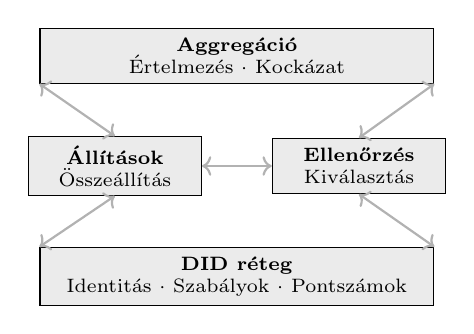
\begin{tikzpicture}[
    layer/.style={draw, minimum height=0.7cm, align=center, font=\scriptsize, fill=black!8},
    arr/.style={<->, thick, gray!60}
]
\node[layer, minimum width=5cm] (agg) at (0,2.8) {\textbf{Aggregáció}\\Értelmezés\ $\cdot$ Kockázat};
\node[layer, minimum width=2.2cm] (claim) at (-1.55,1.4) {\textbf{Állítások}\\Összeállítás};
\node[layer, minimum width=2.2cm] (verif) at (1.55,1.4) {\textbf{Ellenőrzés}\\Kiválasztás};
\node[layer, minimum width=5cm] (did) at (0,0) {\textbf{DID réteg}\\Identitás $\cdot$ Szabályok $\cdot$ Pontszámok};

\draw[arr] (agg.south west) -- (claim.north);
\draw[arr] (agg.south east) -- (verif.north);
\draw[arr] (claim.east) -- (verif.west);
\draw[arr] (claim.south) -- (did.north west);
\draw[arr] (verif.south) -- (did.north east);
\end{tikzpicture}
\caption{Az RSN négyrétegű architektúrája.}
\label{fig:architecture}
\end{figure}

\subsection{A résztvevők szerepei}

Egy ellenőrzési tranzakcióban legfeljebb hat különálló DID szerep vesz részt (\ref{fig:roles}.~ábra): \textbf{kibocsátó} ($DID_I$, létrehozza és benyújtja az állítást), \textbf{alany} ($DID_S$, az a DID, amelyről az állítás szól---egybeeshet a kibocsátóval), \textbf{tekintély} ($DID_A$, díj ellenében jóváhagyja az állítást; tanúszolgálatot is kínálhat---\emph{opcionális}), \textbf{tanú} ($DID_{W_{1..n}}$, az ellenőr becsületességének inkognitó megfigyelője kihívási kódokon keresztül---\emph{opcionális}), \textbf{ellenőr} ($DID_V$, algoritmikusan kiválasztva az állítás közzétételére), valamint az \textbf{RSN} (a hálózat, ahol az ellenőrzött állítások megjelennek). Bármely szerep átruházható egy másik DID-re (7.4.~szakasz). Egy tekintély gyakran a jóváhagyást tanúszolgálattal csomagolja össze, ám a két funkció logikailag független.

\begin{figure}[ht]
\centering
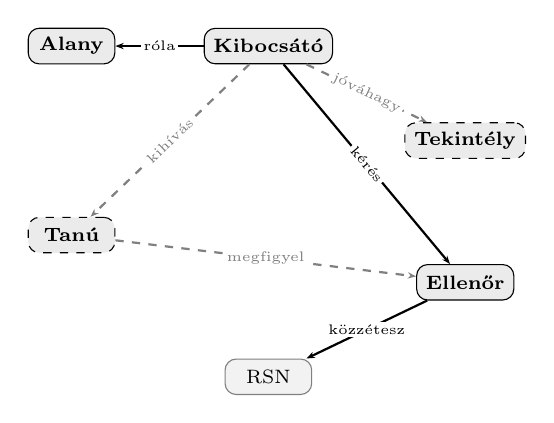
\begin{tikzpicture}[
    role/.style={draw, rounded corners, minimum width=1.1cm, minimum height=0.45cm, align=center, font=\scriptsize, fill=black!8},
    opt/.style={draw, rounded corners, minimum width=1.1cm, minimum height=0.45cm, align=center, font=\scriptsize, fill=black!8, dashed},
    arr/.style={-{Stealth[length=3pt]}, thick},
    oarr/.style={-{Stealth[length=3pt]}, thick, dashed, gray},
    lbl/.style={font=\tiny, fill=white, inner sep=1pt}
]
\node[role] (I) at (0,2.4) {\textbf{Kibocsátó}};
\node[role] (S) at (-2.5,2.4) {\textbf{Alany}};
\node[opt] (A) at (2.5,1.2) {\textbf{Tekintély}};
\node[opt] (W) at (-2.5,0) {\textbf{Tanú}};
\node[role] (V) at (2.5,-0.6) {\textbf{Ellenőr}};
\node[role, fill=black!5, draw=gray] (N) at (0,-1.8) {RSN};

\draw[arr] (I) -- node[lbl] {róla} (S);
\draw[oarr] (I) -- node[lbl,sloped] {jóváhagy} (A);
\draw[oarr] (I) -- node[lbl,sloped] {kihívás} (W);
\draw[arr] (I) -- node[lbl,sloped] {kérés} (V);
\draw[oarr] (W) -- node[lbl] {megfigyel} (V);
\draw[arr] (V) -- node[lbl] {közzétesz} (N);
\end{tikzpicture}
\caption{DID szerepek egy ellenőrzési tranzakcióban. Szaggatott = opcionális (tekintély, tanú).}
\label{fig:roles}
\end{figure}

\subsection{Megvesztegethetetlenség: négy erő}

Az RSN megvesztegethetetlensége nem egyetlen mechanizmusból fakad, hanem négy egyidejűleg ható erőből. Egyik sem elegendő önmagában; csak együttesük teszi a korrupciós kísérletet gazdaságilag irracionálissá.

\textbf{Kiszámíthatatlan célpont.} Az egyes állítások ellenőrét nemdeterminisztikusan, konzisztens hasítással választják ki (5.3.~szakasz). A támadó nem tud előre megcélozni egy adott ellenőrt megvesztegetés céljából, mert az ellenőr kiléte az állítás tartalmának és a korábbi iterációknak a függvénye, nem a kibocsátó választásáé.

\textbf{Reputációs tőkeáttétel---lassan fel, gyorsan le.} A reputáció csak fokozatosan, tartósan következetes viselkedés révén szerezhető meg. Ám katasztrofálisan elveszíthető egyetlen csalárd jóváhagyással (6.2.~szakasz). Ez az aszimmetria azt jelenti, hogy évek alatt felhalmozott reputációt egyetlen tisztességtelen jóváhagyás lerombolhat; az optimális stratégia továbbra is a gyanús állítások elutasítása marad.

\textbf{Nyilvános ígéret.} Minden DID-birtokos nyilvánosan deklarálja a szabályzatát---egy géppel olvasható szabálykészletet, amelynek betartására kötelezettséget vállal. A deklaráció és a tényleges viselkedés közötti eltérés kimutatható, és az alapul szolgáló szabálysértésnél súlyosabb reputációs vétségként áraztatik be (7.3.~szakasz). A képmutatás ezért drágább, mint a közvetlen tisztességtelenség.

\textbf{Háló-támadási költség aszimmetriája.} A hálózat cenzúrázásának vagy destabilizálásának költsége nemlineárisan nő a hálózat méretével és sűrűségével, míg az eltűrésének költsége állandó marad. Ahhoz, hogy a cenzúra kifizetődő legyen, egy központosított szereplőnek az egész hálózatra ki kellene terjesztenie azt---olyan intézkedéseket követelve, amelyek aránytalanok bármely elképzelhető haszonnal (10.~szakasz).

% ============================================================
% 4. DECENTRALIZED IDENTITY MODEL
% ============================================================
\section{Decentralizált identitásmodell}

\subsection{DID különleges tulajdonságokkal}

Az RSN a W3C DID Core specifikációt~\cite{did2022} a következőkkel egészíti ki: \textbf{deklarált szabályok} (géppel olvasható viselkedési kötelezettségvállalások), \textbf{reputációs metaadatok} (aggregált viselkedési pontszám), valamint \textbf{hálózati útválasztás} (változtatható onion átjáró, amely elkülönül a stabil gyűrűpozíciótól).

\subsection{Az állítás életciklusa}

Egy állítás hat szakaszon halad át (\ref{fig:lifecycle}.~ábra): összeállítás, opcionális tekintélyi jóváhagyás, ellenőr-kiválasztás konzisztens hasítással, ellenőrzési döntés (elfogadás vagy elutasítás iterációval), közzététel, valamint reputáció-frissítés minden fél számára.

\begin{figure}[ht]
\centering
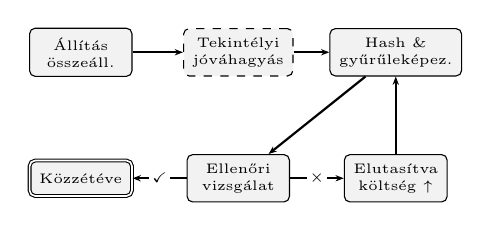
\begin{tikzpicture}[
    stp/.style={draw, rounded corners=2pt, minimum width=1.3cm, minimum height=0.45cm, align=center, font=\tiny, fill=black!5},
    arr/.style={-{Stealth[length=3pt]}, thick},
    lbl/.style={font=\tiny, fill=white, inner sep=1pt}
]
\node[stp] (comp) at (0,0) {Állítás\\összeáll.};
\node[stp, dashed] (auth) at (2.0,0) {Tekintélyi\\jóváhagyás};
\node[stp] (hash) at (4.0,0) {Hash \&\\gyűrűleképez.};
\node[stp] (ver) at (2.0,-1.6) {Ellenőri\\vizsgálat};
\node[stp, double] (pub) at (0,-1.6) {Közzétéve};
\node[stp] (rej) at (4.0,-1.6) {Elutasítva\\költség $\uparrow$};

\draw[arr] (comp) -- (auth);
\draw[arr] (auth) -- (hash);
\draw[arr] (hash) -- (ver);
\draw[arr] (ver) -- node[lbl] {\checkmark} (pub);
\draw[arr] (ver) -- node[lbl] {$\times$} (rej);
\draw[arr] (rej) -- ++(0,0.8) -| (hash);
\end{tikzpicture}
\caption{Az állítás életciklusa iterációs hurokkal.}
\label{fig:lifecycle}
\end{figure}

\subsection{Kapcsolat a W3C DID Core specifikációval}

Az RSN identitásmodellje a W3C DID Core specifikáció~\cite{did2022} valódi bővebb halmaza. Minden RSN DID érvényes W3C DID. Az RSN-specifikus kiterjesztéseket egy dedikált DID-metódus specifikációban meghatározott DID-dokumentumtulajdonságokként kódolják, ami kompatibilis a meglévő infrastruktúrával, például az ION~\cite{buchner2021} és a Ceramic~\cite{ceramic2023} rendszerekkel.

% ============================================================
% 5. VERIFICATION AND PROPAGATION
% ============================================================
\section{Az információ ellenőrzése és terjesztése}

\subsection{Az információbevitel költsége}

Az RSN alapvető gazdasági elve az olvasás és az írás közötti aszimmetria. A reputációs adatok olvasása nulla határköltséghez közelít azon résztvevők számára, akik a DID-hálózat részei, és reputációjukkal arányos hozzáféréssel rendelkeznek---az újonnan érkezőknek fokozatosan ki kell érdemelniük a szélesebb hozzáférést (lásd a potyautas-védelmet). Az írás---úgy értve, mint a reputáció tartós materializálódása a hálózatba, nem pedig egyszeri technikai aktus---ellenőrizhető, halmozódó ráfordítást igényel három dimenzióban: \textbf{idő} (a következetes viselkedésre, a teljesített kötelezettségvállalásokra és az ápolt kapcsolatokra fordított életévek), \textbf{energia} (a becsületes ügyintézésbe, a partnerségek gondozásába és a hosszú távú megbízhatóságba fektetett erőfeszítés), valamint \textbf{pénz} (a saját név javára történő befektetés---szakmai fejlődés, a munka minősége, az okozott károk jóvátétele). A reputáció nem vásárolható meg azonnal---az egész életen át tartó felhalmozódás eredménye, amelyet a rendszer csupán láthatóvá és a kontextusok között átvihetővé tesz. A protokoll egyszeri technikai költségei (kriptográfiai aláírások, ellenőri díjak) elhanyagolhatók ehhez az alapul szolgáló befektetéshez képest.

\subsection{Társadalmi gráf és kapcsolati mélység}

Az RSN alapvetően egy közösségi hálózat: minden DID kontaktokat (más DID-eket) ad hozzá, akik engedélyezik a kapcsolatot. Ezeknek a kontaktoknak megvannak a saját kontaktjaik, és így tovább. Az algoritmikus ellenőrkeresés a kapcsolt kontaktok konfigurálható $h$ mélységén belül működik (pl. $h=3$: a közvetlen kontaktok, azok kontaktjai, és a kontaktok kontaktjai). Ez az architektúra nem igényel egyetlen globális blokkláncot---természetesen kedvez a közösségek/klaszterek kialakulásának, amelyek átfednek más közösségekbe. Minden DID-résztvevőnek rendelkeznie kell közzétett \textbf{szabályzattal}---egy géppel olvasható szabálykészlettel, amely szabályozza, hogyan értékelik a beérkező kéréseket. A szabályzatsértéseket a hálózat negatív artefaktumokként rögzíti.

\subsection{Algoritmikus ellenőr-kiválasztás}

Az ellenőrzési protokoll konzisztens hasítást~\cite{karger1997} alkalmaz (\ref{fig:verifier}.~ábra). Az ellenőrzés fizetett szolgáltatás: az ellenőrök díjért működnek, létrehozva egy piacot, ahol a verseny formálja az árazást, a sebességet és a megbízhatóságot.

\textbf{1. lépés.} Az állítási dokumentumot összefűzik az előző iteráció hasítási eredményével (vagy $\varnothing$-vel az első iterációnál), és hasítják:
\begin{equation}
\text{pos} = f_h(\text{claim} \| \text{prev\_hash})
\label{eq:hash}
\end{equation}

Az algoritmusnak tartalmaznia kell az összes korábbi kérés és válasz \emph{teljes útvonalát}---nem pusztán az előző iteráció hasítását. Minden ellenőr teljes válasza (elfogadás, elutasítás, megadott ár, indoklás) hozzáfűződik a növekvő dokumentumhoz, amely minden lépésnél kriptográfiai aláírásokkal ellenőrizhető.

\textbf{2. lépés.} A hasítást leképezik a konzisztens hasítási gyűrűn $N$ pozícióra, egyenletesen elosztva (pl. $N=4$ esetén: $+0^{\circ}, +90^{\circ}, +180^{\circ}, +270^{\circ}$). Minden pozícióból egy óramutató járásával megegyező irányú keresés választja ki a legközelebbi DID-et ellenőrjelöltként (\ref{fig:multipoint}.~ábra). Az $N$ egy változó paraméter, amely függhet a jelenleg aktív DID-ek százalékos arányától, a napszaktól vagy a hálózat korábbi reakciókészségétől.

\textbf{3. lépés.} Az ellenőr elfogad (közzétesz, reputációt téve fel) vagy elutasít (visszatérve az 1.~lépéshez az elutasítás hasításával). Amikor egy csomópont nem válaszol annak ellenére, hogy online állapotot deklarál, a következő kérésnek tartalmaznia kell mind az $N$ korábbi ellenőrjelölt összes válaszát.

\textbf{Potyautas-védelem.} A cél-DID-ek díjakat vagy hozzáférési korlátozásokat állíthatnak be a kevés reputációval rendelkező új DID-ek lekérdezéseihez. Ez a fokozatos (nem bináris) mechanizmus arra kényszeríti az újonnan érkezőket, hogy valós tevékenységgel építsenek reputációt, mielőtt szabadon fogyaszthatnák mások adatait.

\begin{figure}[ht]
\centering
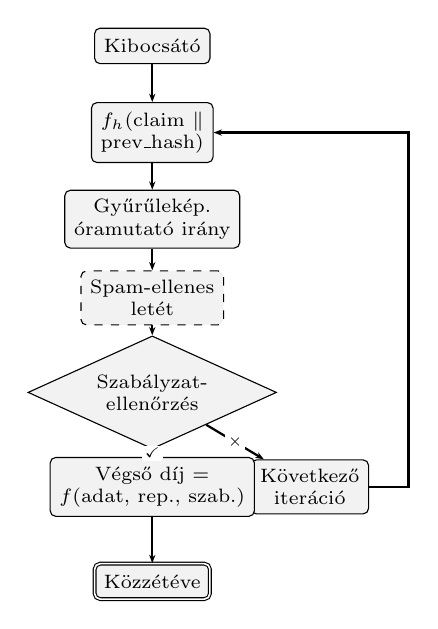
\begin{tikzpicture}[
    box/.style={draw, rounded corners=2pt, minimum width=1.3cm, minimum height=0.45cm, align=center, font=\scriptsize, fill=black!5},
    dec/.style={draw, diamond, aspect=2.2, minimum width=0.9cm, align=center, font=\scriptsize, fill=black!5},
    arr/.style={-{Stealth[length=3pt]}, thick},
    lbl/.style={font=\tiny, fill=white, inner sep=1pt}
]
\node[box] (iss) at (0,0) {Kibocsátó};
\node[box] (hash) at (0,-1.1) {$f_h$(claim $\|$\\prev\_hash)};
\node[box] (ring) at (0,-2.2) {Gyűrűlekép.\\óramutató irány};
\node[box, dashed] (spam) at (0,-3.2) {Spam-ellenes\\letét};
\node[dec] (check) at (0,-4.4) {Szabályzat-\\ellenőrzés};
\node[box] (rej) at (2,-5.6) {Következő\\iteráció};
\node[box] (fee) at (0,-5.6) {Végső díj =\\$f$(adat, rep., szab.)};
\node[box, double] (pub) at (0,-6.8) {Közzétéve};

\draw[arr] (iss) -- (hash);
\draw[arr] (hash) -- (ring);
\draw[arr] (ring) -- (spam);
\draw[arr] (spam) -- (check);
\draw[arr] (check) -- node[lbl] {$\times$} (rej);
\draw[arr] (check) -- node[lbl] {\checkmark} (fee);
\draw[arr] (fee) -- (pub);
\draw[arr] (rej.east) -- ++(0.5,0) |- (hash.east);
\end{tikzpicture}
\caption{Ellenőr-kiválasztási protokoll. A spam-ellenes letét opcionális és visszatéríthető lehet. A végső díjat csak elfogadás esetén fizetik.}
\label{fig:verifier}
\end{figure}

Minden elutasítás hozzáfűzi az ellenőr teljes válaszát (az indokokat és feltételeket is beleértve) az állítási dokumentumhoz, kibővítve annak tartalmát. A kibővített dokumentumból nemdeterminisztikusan új hasítást számítanak, amely egy másik gyűrűpozícióra képeződik le, és egy másik ellenőrt választ ki. A teljes útvonal dokumentálása kötelező---a kibocsátó nem tudja megjósolni vagy befolyásolni a következő ellenőrt. Ha egy ellenőr figyelmen kívül hagy egy kérést kompatibilis deklarált szabályzat ellenére, a tanúk (ha jelen vannak) ezt rögzítik, és a kibocsátó a végső közzétételkor csatolhatja a tanúbizonyítékot.

\begin{figure}[ht]
\centering
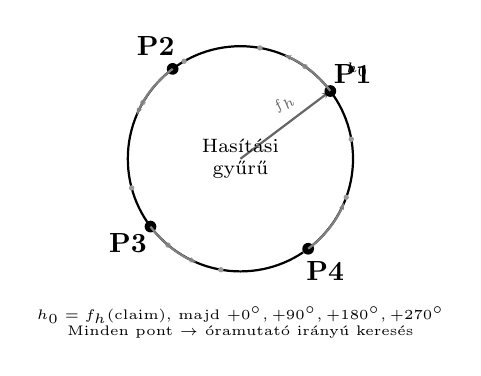
\begin{tikzpicture}[scale=0.65]
% Ring
\draw[thick] (0,0) circle (2.2cm);
% DID nodes on ring
\foreach \a in {10,55,80,120,150,195,230,260,305,340} {
  \fill[black!40] (\a:2.2) circle (1.5pt);
}
% Hash offset arrow pointing to initial position
\draw[-{Stealth[length=3pt]}, thick, black!60] (0,0) -- node[font=\tiny,above,sloped,pos=0.6] {$f_h$} (37:2.2);
\fill[black] (37:2.2) circle (2pt);
\node[font=\tiny,anchor=south west] at (37:2.35) {$h_0$};
% N=4 points offset from h0 by +0, +90, +180, +270
\foreach \offset/\l in {0/P1,90/P2,180/P3,270/P4} {
  \pgfmathsetmacro{\ang}{37+\offset}
  \node[fill=black, circle, inner sep=1.5pt] (p\offset) at (\ang:2.2) {};
  \node[font=\tiny,font=\bfseries] at (\ang:2.75) {\l};
  % clockwise search arc
  \draw[-{Stealth[length=2.5pt]}, thick, gray] (\ang:2.2) arc (\ang:\ang+30:2.2);
}
\node[font=\scriptsize, align=center] at (0,0) {Hasítási\\gyűrű};
\node[font=\tiny, align=center] at (0,-3.2) {$h_0 = f_h(\text{claim})$, majd $+0^{\circ},+90^{\circ},+180^{\circ},+270^{\circ}$\\Minden pont $\rightarrow$ óramutató irányú keresés};
\end{tikzpicture}
\caption{Többpontos kiválasztás ($N{=}4$). A $h_0$ hasítás adja az eltolást; 4 pont egyenletesen elosztva $h_0$-tól.}
\label{fig:multipoint}
\end{figure}

\subsection{Tanúprotokoll}

A \textbf{tanú} szerep inkognitó elszámoltathatóságot biztosít az ellenőr becsületessége felett egy kriptográfiai kihívási-kód protokollon keresztül:

\textbf{W1. lépés.} A kérelmező aláírja az ellenőrzési kérést, és elküldi $N_w$ tanúnak---kontaktoknak a kérelmező közösségi hálózatából, vagy díj ellenében működő szakosodott tanúszolgálat-nyújtóknak.

\textbf{W2. lépés.} Minden $w_i$ tanú aláírja a teljes aláírt kérést, megőrzi az eredeti $\sigma_i$ aláírást, és kiszámít egy $c_i = h(\sigma_i)$ kihívási kódot. A kihívási kód hozzáfűződik a kéréshez.

\textbf{W3. lépés.} A kérés, amely immár $N_w$ kihívási kódot hordoz, elküldésre kerül az ellenőrnek. Az ellenőr megfigyeli a kódokat, de \emph{nem tudja megállapítani}, kik a tanúk, vagy hogy a kódok valós aláírásoknak felelnek-e meg.

\textbf{W4. lépés (becsületes ellenőr).} Ha az ellenőr a deklarált szabályzatának megfelelően válaszol, a kihívási kódok átláthatatlanok maradnak. A tanúk sosem lepleződnek le. Nem tesznek közzé további adatot.

\textbf{W5. lépés (szabályzatsértés).} Ha az ellenőr megsérti a szabályzatát (figyelmen kívül hagyja a kérést, inkonzisztensen válaszol), a kérelmező birtokolja a tanúk eredeti $\sigma_i$ aláírásait. Ezek kísérő adatként közzétehetők: bárki ellenőrizheti, hogy $c_i = h(\sigma_i)$, bizonyítva, hogy a tanú jelen volt. A kérelmező függetlenül közzéteheti---az ellenőr már aláírta a kihívási kódokat a válaszában.

\textbf{A blöff tulajdonság.} A kérelmező néhány vagy az összes kihívási kód helyett véletlen értékeket helyettesíthet be. Az ellenőr nem tudja megkülönböztetni a valódi kódokat (magas reputációjú tekintélyek által fedezetteket) a zajtól. Ez a \emph{bizonytalanság} az érvényesítési mechanizmus: minden kérés magában hordozza annak kockázatát, hogy egy tekintélyes hatóság inkognitó figyeli. E nyomás fenntartásának költsége közel nulla (véletlen számok generálása), miközben a tisztességtelenség lehetséges költsége az ellenőr számára katasztrofális. A becsületes viselkedés még tényleges tanúk hiányában is ösztönözve van.

\textbf{Tekintély mint tanú.} Egy tekintély, amely jóváhagy egy állítást, tanúszolgálatot is csomagolhat hozzá: ,,jóváhagyom az állításodat, és inkognitó tanúként szolgálok az ellenőrzés során''. Ez természetes üzleti modell---a tekintély már rendelkezik kontextussal. A két szerep azonban logikailag független.

\subsection{A drága radikalizmus elve}

Három költségcsatorna erősíti egymást egyidejűleg (\ref{fig:radicalism}.~ábra):

\textbf{1. csatorna: iterációs költség.} Minden elutasítás egy új iterációt kényszerít ki, amely időt és erőforrásokat emészt fel. Lineáris növekedés.

\textbf{2. csatorna: dokumentumduzzadás.} Minden iteráció hozzáadja az ellenőr teljes válaszát az állítási dokumentumhoz. A növekedés lineáris, de alapeltolással: a kezdeti hasznos teher (az állítás tartalma, a tekintélyi jóváhagyás, a kriptográfiai aláírások) már nem elhanyagolható $B_0$ mérettel rendelkezik. Teljes méret $k$ iteráció után: $S(k) = B_0 + k \cdot \Delta$, ahol $\Delta$ az átlagos válaszméret.

\textbf{3. csatorna: ellenőri kockázati felár.} A kockázat szubjektív. Az ellenőr felméri, hogy a kérelmező DID deklarált szabályzatai ütköznek-e az ellenőr saját kereskedelmi, társadalmi vagy politikai érdekeivel. A felár exponenciálisan nőhet az ellenőr ,,ideáljától'' észlelt távolsággal: $P(d) = \alpha \cdot e^{\beta d}$, ahol $d$ az ellenőr szubjektív távolságmértéke. Egy személyes tiltott határon túl az ellenőr teljesen megtagadhatja.

\begin{figure}[ht]
\centering
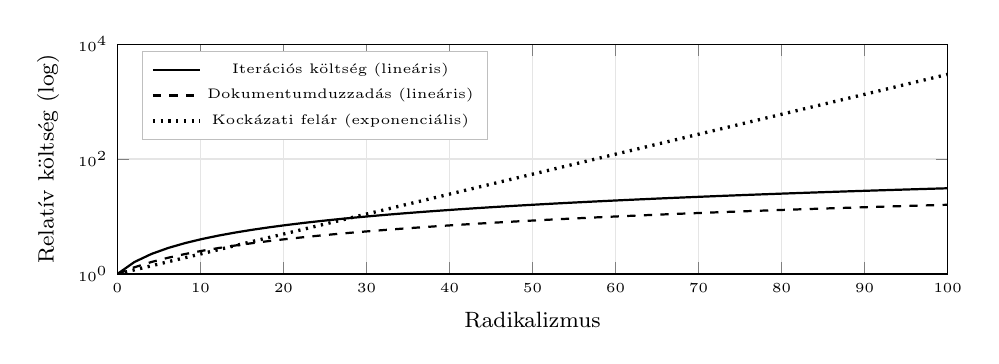
\begin{tikzpicture}
\begin{axis}[
    width=\columnwidth,
    height=4.5cm,
    xlabel={\footnotesize Radikalizmus},
    ylabel={\footnotesize Relatív költség (log)},
    ymode=log,
    xmin=0, xmax=100,
    ymin=1, ymax=10000,
    grid=major,
    grid style={gray!20},
    legend style={at={(0.03,0.97)},anchor=north west,font=\tiny,draw=gray!50},
    tick label style={font=\tiny},
    label style={font=\footnotesize},
]
\addplot[black, thick, domain=0:100, samples=50] {1 + 0.3*x};
\addlegendentry{Iterációs költség (lineáris)}
\addplot[black, thick, dashed, domain=0:100, samples=50] {1 + 0.15*x};
\addlegendentry{Dokumentumduzzadás (lineáris)}
\addplot[black, thick, dotted, line width=1.2pt, domain=0:100, samples=100] {exp(0.08*x)};
\addlegendentry{Kockázati felár (exponenciális)}
\end{axis}
\end{tikzpicture}
\caption{Költségeszkaláció három csatornán át. A kockázati felár dominál magas radikalizmusnál.}
\label{fig:radicalism}
\end{figure}

Lényeges, hogy ez nem cenzúra. Egyetlen állítás sincs megtiltva. A rendszer beárazza a kockázatot (\ref{tab:costs}.~táblázat).

\begin{table}[ht]
\centering
\caption{Költség-összehasonlítás az állítástípusok között.}
\label{tab:costs}
\footnotesize
\begin{tabular}{@{}lcccc@{}}
\toprule
\textbf{Típus} & \textbf{Iter.} & \textbf{Dok.} & \textbf{Díj} & \textbf{Összes} \\
\midrule
Hiteles & $k_{\min}$ & $B_0$ & $P_{\min}$ & Alacsony \\
Ellentmondásos & $k_{\text{med}}$ & $B_0{+}k\Delta$ & $\alpha e^{\beta d}$ & Mérsékelt \\
Radikális & $k_{\max}$ & $\gg B_0$ & $\gg P_{\min}$ & Nagyon magas \\
Csalárd & $\to\infty$ & --- & --- & Közzétehetetlen \\
\bottomrule
\end{tabular}
\end{table}

% ============================================================
% 6. REPUTATION AND RISK
% ============================================================
\section{Reputáció és kockázatértékelés}

\subsection{Reputáció-felhalmozási modell}

A reputáció három tulajdonságot mutat: \textbf{lassú felhalmozódás} (fokozatos növekedés következetes viselkedés révén), \textbf{gyors lerombolás} (egyetlen csalás katasztrofálisan csökkentheti a pontszámot), valamint \textbf{egyéni értékelés} (minden fogyasztó fél a saját aggregációs függvényét alkalmazhatja).

\subsection{Reputábilis tekintélyek}

Egy reputábilis tekintély átvizsgálja az állításokat, és ha meggyőződött, társaláírja őket---saját reputációját téve fel (\ref{fig:authority}.~ábra). Az aszimmetria szándékos: a reputáció megszerzése lassú (fokozatos $+\delta$ becsületes jóváhagyásonként), miközben elvesztése katasztrofális ($-\Delta \gg \delta$ hamis jóváhagyásonként; szemléltetésképp pl. $+2\%$ vs.\ $-70\%$). Az optimális stratégia mindig a gyanús állítások elutasítása. A $\delta$ és $\Delta$ konkrét értékei rendszerparaméterek.

\begin{figure}[ht]
\centering
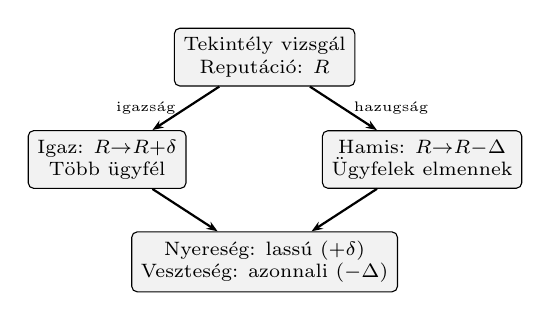
\begin{tikzpicture}[
    box/.style={draw, rounded corners=2pt, minimum width=2cm, minimum height=0.6cm, align=center, font=\scriptsize, fill=black!5},
    arr/.style={-{Stealth[length=4pt]}, thick}
]
\node[box] (exam) at (0,0) {Tekintély vizsgál\\Reputáció: $R$};
\node[box] (true) at (-2,-1.3) {Igaz: $R{\to}R{+}\delta$\\Több ügyfél};
\node[box] (false) at (2,-1.3) {Hamis: $R{\to}R{-}\Delta$\\Ügyfelek elmennek};
\node[box] (insight) at (0,-2.6) {Nyereség: lassú ($+\delta$)\\Veszteség: azonnali ($-\Delta$)};

\draw[arr] (exam) -- node[left,font=\tiny] {igazság} (true);
\draw[arr] (exam) -- node[right,font=\tiny] {hazugság} (false);
\draw[arr] (true) -- (insight);
\draw[arr] (false) -- (insight);
\end{tikzpicture}
\caption{Reputábilis tekintély---aszimmetrikus ösztönzők.}
\label{fig:authority}
\end{figure}

\subsection{Többdimenziós reputáció}

A reputáció nem skalár, hanem vektor több dimenzió mentén: pénzügyi megbízhatóság, személyes integritás, szakmai kompetencia, közéleti szerepvállalás és mások (\ref{fig:reputation-radar}.~ábra). A különböző értékelést nyújtó szolgáltatók ezt a vektort másképp vetítik ki a kontextustól függően---egy hitelező a pénzügyi megbízhatóságot helyezi előtérbe, egy munkáltató a szakmai kompetenciát, egy szomszéd a közéleti viselkedést. Nincs egyetlen ,,helyes'' reputációs pontszám; csak nézőpontok.

\begin{figure}[ht]
\centering
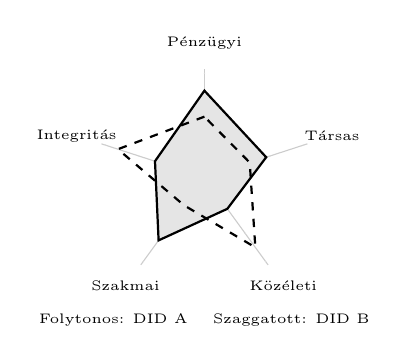
\begin{tikzpicture}[scale=0.55]
\foreach \a/\l in {90/Pénzügyi,162/Integritás,234/Szakmai,306/Közéleti,18/Társas} {
  \draw[gray!40] (0,0) -- (\a:2.5);
  \node[font=\tiny, align=center] at (\a:3.1) {\l};
  \foreach \r in {0.8,1.6,2.4} {
    \fill[black!15] (\a:\r) circle (0.5pt);
  }
}
\draw[thick, fill=black!10] (90:2.0) -- (162:1.2) -- (234:1.8) -- (306:0.9) -- (18:1.5) -- cycle;
\draw[thick, dashed] (90:1.4) -- (162:2.1) -- (234:0.8) -- (306:2.0) -- (18:1.1) -- cycle;
\node[font=\tiny] at (0,-3.3) {Folytonos: DID A \quad Szaggatott: DID B};
\end{tikzpicture}
\caption{Többdimenziós reputációs vektorok. A különböző DID-ek eltérő profilokat mutatnak a dimenziók mentén.}
\label{fig:reputation-radar}
\end{figure}

\subsection{Demokratizált kockázatértékelés}

Az RSN demokratizálja a szisztematikus kockázatértékelést---egy olyan képességet, amely jelenleg a pénzügyi intézményekben összpontosul, ám a bankszektoron messze túl is alkalmazható. Ipari konglomerátumok a beszállítói megbízhatóság felmérésekor, biztosítótársaságok a viselkedési kockázat árazásakor, átvilágítás fúziók és felvásárlások esetén, berendezések élettartamának becslése a gyártásban---bárhol, ahol az ellenféllel kapcsolatos kockázatot fel kell mérni, az RSN decentralizált, piaci alapú alternatívát kínál. Az értelmezési szolgáltatások piaca a nyers, többdimenziós reputációs adatokat cselekvésre alkalmas összefoglalókká fordítja, elérhetővé téve az ellenfél értékelését bármely résztvevő számára határköltségen.

% ============================================================
% 7. CONSENSUS AND DISPUTE RESOLUTION
% ============================================================
\section{Konszenzus és vitarendezés}

\subsection{Decentralizált igazságszolgáltatási modell}

Az RSN az igazságszolgáltatást kétoldalú tárgyalási problémaként fogalmazza újra. A tartós, ellenőrizhető reputációs kár fenyegetése hatékonyabb visszatartó erő, mint egy olyan bírósági eljárás, amelyet a sérelmet elszenvedő fél nem engedhet meg magának.

\subsection{Emergens konszenzus}

Minden résztvevő fenntart egy személyes elégedettségi küszöböt. A hálózat összesített konszenzusa több ezer kétoldalú tárgyalás statisztikai átlagaként emelkedik ki (\ref{fig:consensus}.~ábra). A konszenzus felett messze járó válasz (barbár) drága a közzététele. A konszenzushoz közeli válasz (arányos) olcsó. A konszenzus nem szabály---árjelzés.

\begin{figure}[ht]
\centering
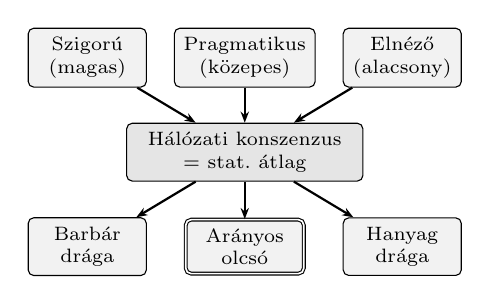
\begin{tikzpicture}[
    person/.style={draw, rounded corners=2pt, minimum width=1.5cm, minimum height=0.5cm, align=center, font=\scriptsize, fill=black!5},
    arr/.style={-{Stealth[length=4pt]}, thick}
]
\node[person] (a) at (-2,0) {Szigorú\\(magas)};
\node[person] (b) at (0,0) {Pragmatikus\\(közepes)};
\node[person] (c) at (2,0) {Elnéző\\(alacsony)};
\node[person, fill=black!10, minimum width=3cm] (cons) at (0,-1.2) {Hálózati konszenzus\\= stat.\ átlag};
\node[person] (exp) at (-2,-2.4) {Barbár\\drága};
\node[person, double] (prop) at (0,-2.4) {Arányos\\olcsó};
\node[person] (neg) at (2,-2.4) {Hanyag\\drága};

\draw[arr] (a) -- (cons);
\draw[arr] (b) -- (cons);
\draw[arr] (c) -- (cons);
\draw[arr] (cons) -- (exp);
\draw[arr] (cons) -- (prop);
\draw[arr] (cons) -- (neg);
\end{tikzpicture}
\caption{Emergens konszenzus egyéni elégedettségi küszöbökből.}
\label{fig:consensus}
\end{figure}

\subsection{A büntetés kalibrálása}

Minden DID-birtokos nyilvánosan deklarálja a válaszait meghatározott vétségkategóriákra. Az aránytalanul szigorú vagy engedékeny deklarációk negatív reputációs jelzéseket vonzanak. Az arányos deklarációkat súrlódás nélkül fogadják el---egy önkalibráló büntetési rendszer.

Maguk a konszenzuális deklarációk is alá vannak vetve a képmutatás-észlelésnek: deklaratívan elkötelezni magunkat egy konszenzuális álláspont mellett, miközben inkonzisztensen viselkedünk, az alapul szolgáló eltérésnél súlyosabb reputációs vétséget képez, mivel szándékos megtévesztést mutat.

\subsection{Delegálás}

Egy DID-en belül minden tevékenység---egyetlen kivétellel---átruházható egy másik DID-re. \textbf{Az alany szerep---az a DID, amelynek viselkedéséről az állítás szól---nem delegálható; nem átruházhatóan kötődik ahhoz az identitásbirtokoshoz, akire az állítás utal.} A többi aktív szerep---kibocsátó, tekintély, tanú, ellenőr---átruházható egy kijelölt meghatalmazott DID-re, akár ellenőrzés, állításbenyújtás, konszenzusban való részvétel vagy vitarendezés céljából. A delegálás bármikor visszavonható. Ez lehetővé teszi a specializációt (pl. szakszerű ellenőrzési szolgáltatások), miközben a birtokos megtartja a végső irányítást és felelősséget. A delegálás az egész rendszerre alkalmazandó, és elengedhetetlen a skálázhatósághoz.

\subsection{Az egyéni erkölcstől az emergens társadalmi szerződésig}

Minden DID deklarált szabályzata az egyéni erkölcs formalizálását képviseli: mit tart a birtokos elfogadhatónak, hogyan reagál meghatározott viselkedésekre, mit követel meg az ellenfelektől. Ezeket a szabályzatokat nem egy rendszertervező írja elő---minden résztvevő maga választja meg és géppel olvasható formában fejezi ki őket.

Ez a formalizálás egy háromszakaszos emergenciát tesz lehetővé. Először az egyéni erkölcs \textbf{szabályzatként} kódolódik---deklarált szabályok, küszöbök és válaszfüggvények halmazaként, amelyek betartására a DID kötelezettséget vállal. Másodszor a hálózat összes szabályzatának összessége \textbf{emergens etikát} hoz létre---statisztikailag megfigyelhető normákat, amelyeket egyetlen résztvevő sem tervezett, de amelyek több ezer egyéni erkölcsi álláspont interakciójából keletkeznek~\cite{durkheim1893}. Harmadszor ezek az emergens etikák, közös viselkedési normákként kifejezve és kétoldalú árjelzéseken keresztül érvényesítve, \textbf{mérhető társadalmi szerződést} képeznek---nem elméleti konstrukciót, amelyet senki sem írt alá~\cite{rawls1971}, hanem a tényleges viselkedéssel alátámasztott, empirikusan megfigyelhető szabálykészletet.

Ez a folyamat tükrözi az erkölcsi alapok elméletének~\cite{haidt2012} eredményeit: az emberi erkölcs intuitív, pluralisztikus és kulturálisan változó. Az RSN nem igényel erkölcsi konszenzust bemenetként; viselkedési konszenzust állít elő kimenetként. Az így létrejövő társadalmi szerződés nem statikus---fejlődik, ahogy a résztvevők csatlakoznak, kilépnek, és a hálózati visszacsatolásra reagálva módosítják szabályzataikat. A klasszikus társadalmiszerződés-elmélettel ellentétben ez a szerződés visszavonható, megfigyelhető és szuverén nélkül érvényesíthető.

% ============================================================
% 8. ECONOMIC MODEL
% ============================================================
\section{Gazdasági modell}

Az előző szakaszok egy eszközt írtak le---az RSN ellenőrzési mechanizmusait, költségszerkezetét és emergens konszenzusát. Ez a szakasz egy módszertant ír le ezen eszköz alkalmazására a költségvetési és kormányzati átmenetre. Az eszköz általános célú; az alábbi módszertan egy lehetséges alkalmazás.

\subsection{Ösztönzőszerkezet}

A reputáció mint tőke közvetlen ösztönzőket teremt a becsületes viselkedésre. Normál működésben a résztvevők természetesen építenek reputációt a mindennapi tranzakciók és a teljesített kötelezettségvállalások révén. Az elsődleges kiadás a \emph{negatív} állításokra esik---a mások által okozott károk rögzítésére. Ez az aszimmetria hasznos, megbízható viselkedést ösztönöz: a becsületesség nem kerül semmi többletbe, míg az ártalmasság dokumentált nyomot hagy, amelyet mások hajlandók fizetni a megőrzéséért. A képmutatás---szabályok deklarálása azok betartása nélkül---a legdrágább kudarcmód, mivel szándékos megtévesztést mutat.

\subsection{Párhuzamos költségvetési rendszer}

Három összetevő tesz lehetővé versenynyomást: (1)~\textbf{egyszerű adó}---egyetlen arányos kulcs kivételek nélkül, kezdetben marginálisan a meglévő tényleges kulcs alatt; (2)~\textbf{elektronikus kiadás-nyilvántartás (Electronic Spending Registration, ESR)}---a cseh EET-modell megfordítása, hogy a polgárok felügyeljék az állami kiadásokat; (3)~\textbf{polgár által irányított adóelosztás}---az első évben néhány százalékkal indulva, és egy évtized után elérve akár az alacsony kétjegyű tartományt, akár a polgár által irányított rendszerre való teljes átállást, az elfogadás ütemétől függően. A tényleges tempó attól függ, milyen gyorsan jelennek meg szabadpiaci alternatívák az állami szolgáltatásokra, valamint az állam hajlandóságától, hogy együttműködjön az átmenettel; az idő függvényének nem kell lineárisnak lennie, és nincs ok arra, hogy felső korlátot szabjunk annak, ahová az elfogadás végül eljuthat.

% ============================================================
% 9. MIGRATION PATH
% ============================================================
\section{Átállási út}

Az átállás három fázison halad át (\ref{fig:migration}.~ábra): \textbf{1. fázis: rárétegzés} (az RSN mint információs réteg, az állam az egyetlen szolgáltató), \textbf{2. fázis: verseny} (az RSN funkcionális alternatívákat kínál, kettős rendszerhasználat), valamint \textbf{3. fázis: átmenet} (az RSN felülmúlja az állami megfelelőket, önkéntes átállás). Az átmenet minden szakaszban visszafordítható.

\begin{figure}[ht]
\centering
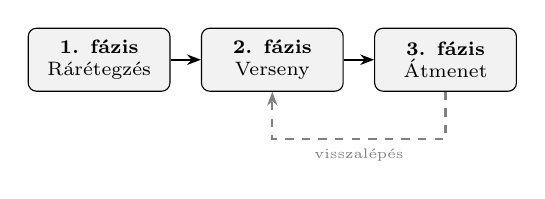
\begin{tikzpicture}[
    phase/.style={draw, rounded corners=3pt, minimum width=1.8cm, minimum height=0.8cm, align=center, font=\scriptsize, fill=black!5},
    arr/.style={-{Stealth[length=5pt]}, thick}
]
\node[phase] (p1) at (0,0) {\textbf{1. fázis}\\Rárétegzés};
\node[phase] (p2) at (2.2,0) {\textbf{2. fázis}\\Verseny};
\node[phase] (p3) at (4.4,0) {\textbf{3. fázis}\\Átmenet};

\draw[arr] (p1) -- (p2);
\draw[arr] (p2) -- (p3);
\draw[arr, dashed, gray] (p3.south) -- ++(0,-0.6) -| node[below,font=\tiny,pos=0.25] {visszalépés} (p2.south);
\end{tikzpicture}
\caption{Háromfázisú átállás---minden szakaszban visszafordítható.}
\label{fig:migration}
\end{figure}

Az elsődleges nyomásmechanizmus költségvetési: amikor a feltételes adófizetők elérnek egy ,,gazdaságilag jelentős kisebbséget $X$''---egy olyan csoportot, amely elég nagy ahhoz, hogy az ellene irányuló elnyomás nem elhanyagolható gazdasági kárt okozzon, és a polgári engedetlenség hiteles fenyegetéssé váljon---az állam tárgyalásba kezd. Szemléltetésül $X \approx 15\%$-nyi GDP-t használunk, de a tényleges küszöb az adott gazdaságtól függ.

% ============================================================
% 10. SECURITY ANALYSIS
% ============================================================
\section{Biztonsági elemzés}

Öt ellenfél-kategóriát tekintünk: egyéni rosszhiszemű szereplők, szervezett csoportok, vállalati ellenfelek, állami szintű ellenfelek, valamint protokollszintű ellenfelek.

\textbf{Sybil-ellenállás}~\cite{douceur2002}. A reputáció felépítése tartós, ellenőrizhető interakciót igényel. Egy sikeres Sybil-támadás költsége lineárisan skálázódik a hamis identitások számával és kvadratikusan a célzott reputációszinttel. Több DID párhuzamos működtetése lehetséges, de szándékosan drága---minden identitásnak önállóan kell reputációt felhalmoznia valós tevékenységgel. Szabad társadalmakban ez a költség elrettent az alkalmi visszaéléstől; diktatúrákban a párhuzamos DID-ek túlélési eszközzé válnak, amelyek lehetővé teszik a részekre bontott ellenállást, a földalatti koordinációt és a biztonságosabb feketepiaci navigálást.

\textbf{Összejátszás elleni védelem.} A zárt csoportokon belüli kölcsönös jóváhagyás mintázatai kimutathatók társadalmi gráfelemzéssel. A reputáció-aggregációs függvények leértékelik a szorosan klaszterezett forrásokból származó állításokat.

\textbf{Állami szintű ellenfél.} Az onion útválasztás, a központosított infrastruktúra hiánya és az ellenőr szerep szétosztása a résztvevők között biztosítja, hogy az elnyomás bármely haszonhoz aránytalan intézkedéseket követel.

\textbf{Adatvédelem vs.\ elszámoltathatóság.} Az álnevűség---köztes út az anonimitás és az identitás felfedése között---lehetővé teszi a DID-ek számára, hogy értékes reputációt halmozzanak fel a birtokos valós identitásának felfedése nélkül.

% ============================================================
% 11. PRIVACY
% ============================================================
\section{Adatvédelmi megfontolások}

Az RSN adatvédelmi modellje az álnevűségre épül. A birtokos irányítja az identitás felfedését: minimális (tiszta álnév), szelektív (meghatározott hitelesítő adatok kapcsolva) vagy teljes (jogi identitás társítva). A közzétett állítások tartósak---a rendszer támogatja a kontextusfüggő helyesbítést, de a törlést nem. Egy birtokos elhagyhat egy kompromittálódott DID-et, és újrakezdheti, feláldozva a felhalmozott reputációt.

% ============================================================
% 12. RELATED WORK
% ============================================================
\section{Kapcsolódó munkák}

A W3C DID Core specifikáció~\cite{did2022} és a Ceramic Network~\cite{ceramic2023} adja az identitásalapot. Az EigenTrust~\cite{kamvar2003} demonstrálta az elosztott reputáció-aggregációt központi hatóság nélkül. Az SBT-k~\cite{weyl2022} bevezették a nem átruházható társadalmi tokeneket. Az RSN abban különbözik, hogy hangsúlyt fektet a gazdasági költségre mint minőségszűrőre, valamint a radikalizmus beárazásának mechanizmusára.

A DAO-k~\cite{buterin2014} és a kvadratikus szavazás~\cite{buterin2019} demonstrálták a decentralizált kormányzás megvalósíthatóságát. Az RSN a konszenzust szavazás helyett kétoldalú áralkukból vezeti le.

A javaslat az anarcho-kapitalista elméletre~\cite{rothbard1973,hoppe2001} támaszkodik a magánszolgáltatás terén, de két kritikus szempontból eltér tőle: a racionalitás feltételezése helyett a rosszindulatra és a megtorlásból fakadó ösztönökre tervez, és forradalom helyett fokozatos átmenetet javasol. Az emergens társadalmi szerződések fogalmának előzményei megtalálhatók Hayek spontán rend elméletében~\cite{hayek1973}.

\textbf{Anarcho-agorizmus.} Az RSN jelentős közös alapot oszt meg az agorista ellengazdaságtannal~\cite{konkin2006}---különösen a párhuzamos intézmények építésének és az önkéntes cserének a hangsúlyozásában. Az agorizmus azonban hajlamos a racionális önérdeket elegendő koordinációs mechanizmusként feltételezni, és gyakran hiányzik belőle egy konkrét átállási út a meglévő állami struktúrákból. Az RSN kifejezetten beépíti a nem racionális viselkedési hajlamokat, és költségvetési nyomásmechanizmust kínál a fokozatos átmenethez.

\textbf{Meritokrácia.} Az RSN talán egy első funkcionális leírását képviseli annak, hogyan emelkedhet ki a meritokrácia~\cite{young1958} rendszerszintű tulajdonságként, nem pedig szlogenként. A hagyományos meritokratikus rendszerek azért vallanak kudarcot, mert egy központi hatóságot igényelnek az ,,érdem'' meghatározásához és érvényesítéséhez. Az RSN-ben az érdem a kétoldalú értékelésekből emelkedik ki: akik értéket teremtenek, reputációt halmoznak fel; egyetlen bizottság sem dönti el, kinek van érdeme.

\textbf{A tulajdon mint privilégium.} Az RSN alapvetően eltér a tulajdonjogok anarcho-kapitalista és osztrák iskolai kezelésétől, amely azokat természetesnek és abszolútnak tekinti. Az RSN keretrendszerében a tulajdon \emph{privilégium}---egy társadalmi elismerés, amely szélsőséges esetekben visszavonható a közösség által, amikor egy résztvevő alapvetően megsérti a közös normákat (árulás, a közösség megvédésének megtagadása egzisztenciális válságban, szisztematikus kizsákmányolás). Ez nem állami kisajátítás, hanem a társadalmi elismerés visszavonása a kétoldalú kapcsolatok hálózata által.

% ============================================================
% 13. LIMITATIONS
% ============================================================
\section{Diszkusszió és korlátok}

\textbf{Hidegindítás.} Az RSN értéke hálózati hatásoktól függ; a korai alkalmazók korlátozott értékkel szembesülnek, amíg a részvétel el nem ér egy küszöböt. Ám már a korai szakaszoktól kezdve a DID-hálózat hasznos kiegészítő információforrásként szolgál. A korai reputációértékelés és tekintélyfelmérés várhatóan fokozatosan, egyre kifinomultabbá válva fejlődik.

\textbf{Potyautas-védelem és hozzáférés-szabályozás.} A cél-DID-ek fokozatos díjakat és hozzáférési korlátozásokat szabhatnak ki az alacsony reputációjú DID-ek lekérdezéseire. Ez nem bináris, hanem folytonos skála: minél kevesebb reputációja van egy lekérdező DID-nek, annál kevesebb információt kap, annál tovább vár, és annál többet fizet. Ez a mechanizmus a valós részvételt ösztönzi a passzív fogyasztással szemben.

\textbf{Hozzáférési egyenlőtlenség.} Az állítások közzétételének költsége kiszűrheti a jogos panaszokat a gazdaságilag hátrányos helyzetű résztvevőktől. Enyhítés: minden résztvevő egyúttal potenciális ellenőrként szolgál (vagy delegálja ezt a szerepet), és ellenőrzési díjakat keres. Elegendő időhorizonton egy nem radikális résztvevőnek meg kell közelítenie a pénzügyi semlegességet---az ellenőrzési bevétel megközelítőleg ellensúlyozza a közzétételi költségeket. Ez statisztikai várakozás, nem garancia.

\textbf{Reputációs egyenlőtlenség.} A korai alkalmazók olyan előnyöket halmoznak fel, amelyek akadályokat teremthetnek a későbbi belépők számára. Ám a reputációértékelést harmadik fél szolgáltatói végzik, akik dönthetnek úgy, hogy aggregációs algoritmusaikkal mérséklik az elsőmozgató-előnyt. Elsőnek lenni jó reputációval legitim komparatív gazdasági előny---és ez szándékos.

\textbf{Nyitott kérdések.} Az optimális költségfüggvények, az aggregációs szabványok, a protokollkormányzás, valamint az MI által generált szintetikus reputációs adatokkal való kölcsönhatás a jövőbeli munka területei maradnak.

Ez a tanulmány nem állítja, hogy az RSN minden körülmények között optimális kimeneteket produkál. Azt állítja, hogy az RSN egy \emph{megvalósítható} alternatívát képvisel---technikailag megvalósítható, gazdaságilag önfenntartó, és társadalmilag összeegyeztethető az emberi viselkedési hajlamokkal úgy, ahogy azok valójában vannak.

% ============================================================
% 14. CONCLUSION
% ============================================================
\section{Következtetés}

Ez a tanulmány bemutatta a reputációs közösségi hálózatot, egy decentralizált protokollt, amely álnéven történő, ellenőrizhető reputációcserét tesz lehetővé. A drága radikalizmus elve biztosítja, hogy a csalárd állítások cenzúra nélkül árazódjanak ki. A javasolt átállási út fokozatos, visszafordítható átmenetet tesz lehetővé a meglévő intézményekből. A terv az emberi természetet olyannak építi be, amilyen---a kicsinyességet, a rosszindulatot és a megtorlásból fakadó elégtétel iránti vágyat is beleértve---ahelyett, hogy ideológiai átalakulást igényelne. Az eredmény nem utópia, hanem egy olyan rendszer, ahol az igazságosság elérhető, a reputáció kiérdemelt, és a vétség költségét az a fél viseli, aki okozta.

% ============================================================
% REFERENCES
% ============================================================
\bibliography{references}

\end{document}
